\documentclass[tikz,border=2pt]{standalone}
\usepackage{amsmath,amssymb}
\usepackage{pgfplots}
\pgfplotsset{compat=1.18}

\begin{document}
% X_n = 1/n: the CDFs are unit steps at 1/n and approach the step at 0, the CDF of the constant 0,
% at every x except the jump point x = 0, where F_n(0) = 0 for all n but F(0) = 1.
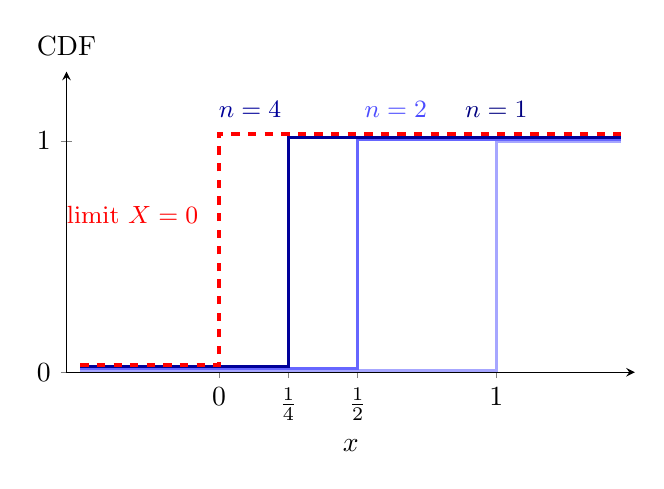
\begin{tikzpicture}
	\begin{axis}[
		axis lines=left, xmin=-0.55, xmax=1.5, ymin=0, ymax=1.3,
		xtick={0,0.25,0.5,1}, xticklabels={$0$,$\tfrac14$,$\tfrac12$,$1$}, ytick={0,1},
		xlabel={$x$}, ylabel={CDF}, ylabel style={rotate=-90, anchor=south, at={(axis description cs:0,1.02)}},
		width=8.8cm, height=5.4cm, clip=false, axis y line=left, axis x line=bottom
		]
		\addplot[blue!35, very thick] coordinates {(-0.5,0.008) (1,0.008) (1,1) (1.45,1)};
		\addplot[blue!60, very thick] coordinates {(-0.5,0.016) (0.5,0.016) (0.5,1.008) (1.45,1.008)};
		\addplot[blue!60!black, very thick] coordinates {(-0.5,0.024) (0.25,0.024) (0.25,1.016) (1.45,1.016)};
		\addplot[red, very thick, dashed] coordinates {(-0.5,0.032) (0,0.032) (0,1.03) (1.45,1.03)};
		\node[blue!50!black, anchor=south, font=\small] at (axis cs:1.0,1.06) {$n=1$};
		\node[blue!70, anchor=south west, font=\small] at (axis cs:0.49,1.06) {$n=2$};
		\node[blue!60!black, anchor=south east, font=\small] at (axis cs:0.26,1.06) {$n=4$};
		\node[red, anchor=south east, font=\small] at (axis cs:-0.04,0.6) {limit $X=0$};
	\end{axis}
	
\end{tikzpicture}
\end{document}
